\documentclass[10pt,a4paper]{article}
% in preamble
\usepackage{animate}
\usepackage{graphics}
%%%%%%%%%%%%%%%%%%%%%%%%%%%
% MODIFY:

\newcommand{\authorA}{ALEX PASQUALI (03754113)}
\newcommand{\authorB}{NICOLA GUGOLE (03753996)}
\newcommand{\groupNumber}{A} % - YOUR GROUP
\newcommand{\exerciseNumber}{4} % - THE NUMBER OF THE EXERCISE
\newcommand{\sourceCodeLink}{\url{https://github.com/AlexPasqua/MLCMS-exercises}}

\newcommand{\workPerAuthor}{
\authorA&Task 1&50\%\\
      &Task 2&50\%\\
      &Task 3&50\%\\
      &Task 4&50\%\\
      \hline
\authorB&Task 1&50\%\\
      &Task 2&50\%\\
      &Task 3&50\%\\
      &Task 4&50\%\\
}

%%%%%%%%%%%%%%%%%%%%%%%%%%%

%%
% imports for the exercise sheets
%

\usepackage[utf8]{inputenc}
\usepackage{amsmath}
\usepackage{amsfonts}
\usepackage{amssymb}

\usepackage[yyyymmdd]{datetime}
\renewcommand{\dateseparator}{--}

\usepackage[left=2cm,right=2cm,top=3cm,bottom=3cm]{geometry}

\usepackage{hyperref}

\usepackage{amsthm}
\newtheorem{lem}{Lemma}
\newtheorem{thm}{Theorem}
\newtheorem{cor}{Corollary}
\newtheorem{rem}{Remark}
\newtheorem{definition}{Definition}
\newtheorem{ter}{Terminology}

\usepackage{graphicx}

\newcommand{\M}{\mathcal{M}}
\newcommand{\N}{\mathcal{N}}
\newcommand{\K}{\mathcal{K}}
\newcommand{\SPDk}{\mathbb{P}^k}
\newcommand{\vol}{\text{vol}}

\newcommand{\Figref}[1]{Figure~\ref{#1}}
\newcommand{\figref}[1]{figure~\ref{#1}}
\newcommand{\Eqnref}[1]{Equation~(\eqref{#1})}
\newcommand{\eqnref}[1]{equation~(\eqref{#1})}

\usepackage{float}
\usepackage{tabularx}

\usepackage{fancyhdr}
\pagestyle{fancy}

\usepackage{totcount}
\newtotcounter{taskCounter}
\newtotcounter{pointCounter}
\newenvironment{task}[1]{\noindent\stepcounter{taskCounter}\textbf{Report on task #1}\smallbreak\hrule\smallbreak}{\smallbreak\hrule\bigbreak}


\title{Report for exercise \exerciseNumber~from group~\groupNumber}

\makeatletter
\let\thetitle\@title
\let\theauthor\@author
\let\thedate\@date
\makeatother

\providecommand{\versiondate}{\today}

\lhead{Exercise sheet \exerciseNumber}
\chead{Master Praktikum: Modelling and Simulation of Crowds WS2019/20}
\rhead{TUM}
\lfoot{Report of Group \groupNumber}
\cfoot{\thepage}
\rfoot{Last compiled: \versiondate}
\renewcommand{\headrulewidth}{0.4pt}
\renewcommand{\footrulewidth}{0.4pt}

\newcommand{\frontpage}{
\begin{center}
\textbf{\thetitle}\\~\\
\end{center}
\begin{table}[H]
\begin{tabular}{ll}
Tasks addressed:&\total{taskCounter}\\
Authors:&\authorA\\
&\authorB\\
&\authorC\\
Last compiled:&\versiondate\\
Source code:&\sourceCodeLink
\end{tabular}
\end{table}
\vfill
The work on tasks was divided in the following way:
\begin{table}[H]
\begin{tabularx}{\textwidth}{X|p{2cm}|p{2cm}}
\workPerAuthor
\end{tabularx}
\end{table}
\newpage
}

\begin{document}

\frontpage

\begin{task}{1, Principal component analysis}
We implemented a "wrapper" function to compute the SVD decomposition that calls the library function \texttt{numpy.linalg.svd} \cite{numpy-svd}.
In addition to that, it makes possible to center the data by simply passing a boolean argument and it returns the 3 matrices U, S and V (instead of U, list of the singular values and V transpose, as numpy's implementation does).
The code of this function is depicted in Figure \ref{fig:code-svd}.
To check the accuracy of the data reconstruction, we used mostly the percentage of energy captured by the principal components that were not set to zero (Eq. \ref{eq:energy}) and the norm of the difference between the original data and the reconstructed one (Eq. \ref{eq:norm-diff-reconstr}).
When reconstructing the data completely, i.e. without setting any singular value to zero, the method was very precise, since the value of the metric of Eq. \ref{eq:norm-diff-reconstr} was in the order of 10^{-15}.

\begin{equation}\label{eq:energy}
    \frac{1}{trace(S^2)}\sum\limits_{i=1}^L \sigma_i^2
\end{equation}

\begin{equation}\label{eq:norm-diff-reconstr}
    \|X - USV^T\|
\end{equation}

Overall, the method was fairly simple to implement and it only took few days to build and test it.

\begin{figure}[h]
    \centering
    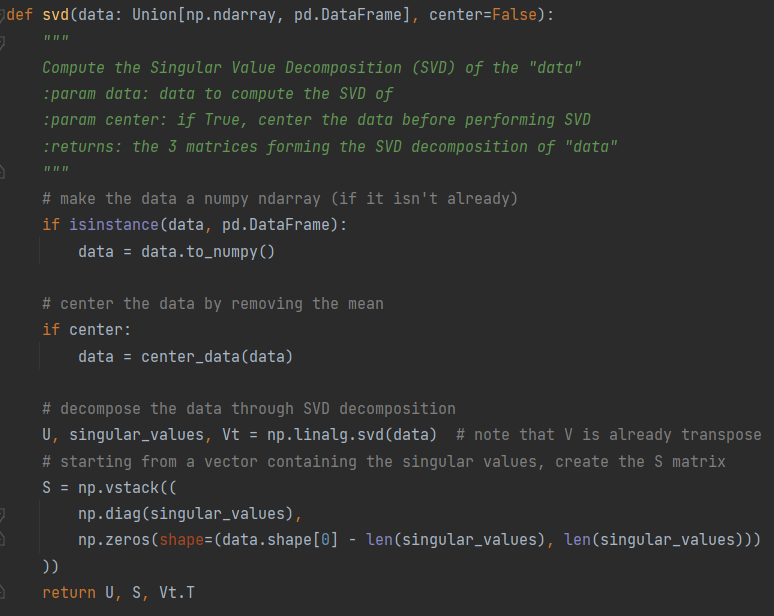
\includegraphics[scale=0.8]{images/code_svd.png}
    \caption{Code of the function implementing the SVD decomposition.}
    \label{fig:code-svd}
\end{figure}

\paragraph{Part 1}
The dataset \texttt{pca\_dataset.txt} contains 2-dimensional data whose scatter plot is shown in Figure \hyperref[fig:scatter-pca-data]{\ref{fig:scatter-pca-data}(a)}.
When computing PCA, in the first principal component it is contained 92.33\% of the energy, while the second one contains only 7.67\% of the total energy.
The directions of the 2 principal components are shown in red in Figure \hyperref[fig:scatter-pca-data]{\ref{fig:scatter-pca-data}(b)}, which is in the original coordinate system.
In order to plot the directions of the principal components with this coordinates system, we plotted 2 lines connecting 2 points: the mean point of the data (which is common to both lines) and the point identified by the first and second column of the matrix V (product of the SVD)
\footnote{When computing the SVD transformation of the data contained in \texttt{pca\_dataset.txt}, the results are the usual 3 matrices U, S and V.
In this case the matrix V has dimensionality 2x2, therefore each of its columns can represent a point in a 2D plane.}.
The code of the function used for this purpose is shown in Figure \ref{fig:plot-principal-components-directions}.

\begin{figure}[H]
    \centering
    \subfloat[a]{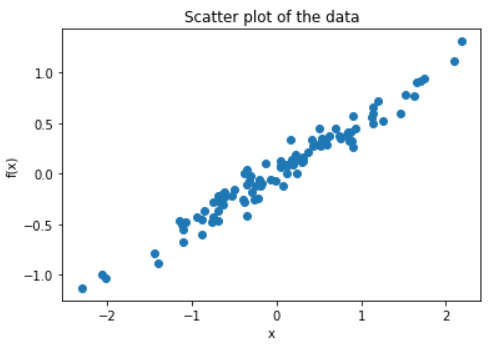
\includegraphics[scale=0.7]{images/scatter_pca_data.png}}
    \hfill
    \subfloat[b]{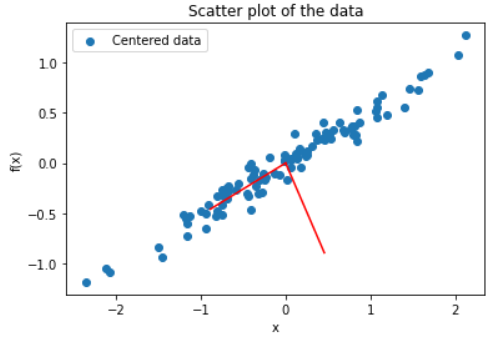
\includegraphics[scale=0.7]{images/scatter_pca_data_with_principal_directions.png}}
    \caption{Scatter plot of the data contained in \texttt{pca\_dataset.txt}.
    (b) shows the plot of the centered data with the directions of the 2 principal components.}
    \label{fig:scatter-pca-data}
\end{figure}

\begin{figure}[H]
    \centering
    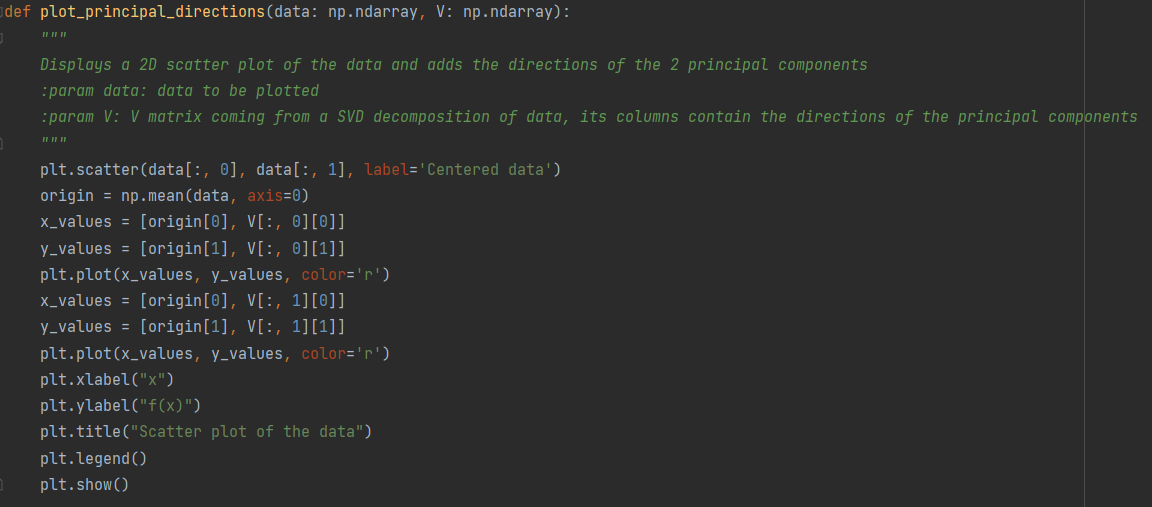
\includegraphics[scale=0.7]{images/plot_principal_components_directions.png}
    \caption{Function used to plot the directions of the 2 principal components of the data contained in \texttt{pca\_dataset.txt}.}
    \label{fig:plot-principal-components-directions}
\end{figure}

\paragraph{Part 2}
In this part it was required to apply PCA to an image of a racoon
\footnote{Available at \url{https://pixnio.com/fauna-animals/raccoons/raccoon-procyon-lotor}}.
The image has been generated using \texttt{scipy.misc.face} \cite{scipy-face}, converted to gray-scale and reshaped to have size (249 x 185).
The columns of the images are considered data points and we applied the PCA to it.
Specifically, we tried to reconstruct the image using all, 120, 50 and 10 principal components and the results are shown in Figure \ref{fig:racoon-recontrs}.\\
With only 50 principal components it is already possible to see some slight differences between the original and reconstructed images, but only with 10 it becomes very evident.
In fact, 120 principal components are enough to capture 99.2\% of the energy (loss is less than 1\%), 50 principal components capture 93.10\% and, finally, 10 principal components only retain 75.76\% of the total energy.\\
Recall that to calculate the percentage of retained energy by a certain number of principal components we used the formula in Eq. \ref{eq:energy}.

\begin{figure}[H]
    \centering
    \subfloat[a]{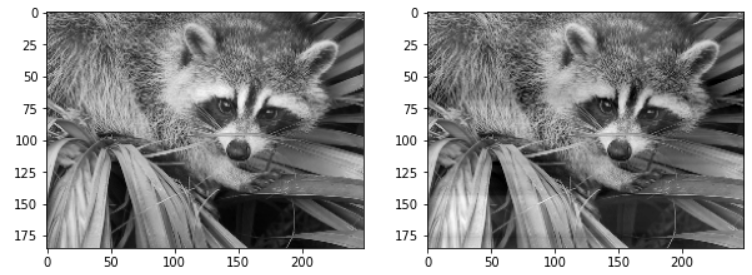
\includegraphics[scale=0.8]{images/racoon_reconstr_all.png}}
    \vfill
    \subfloat[b]{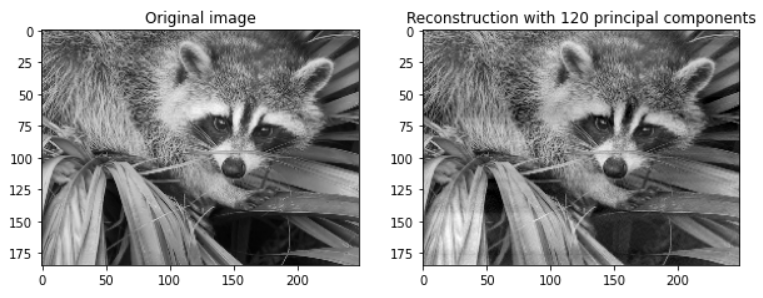
\includegraphics[scale=0.8]{images/racoon_reconstr_120.png}}
    \vfill
    \subfloat[b]{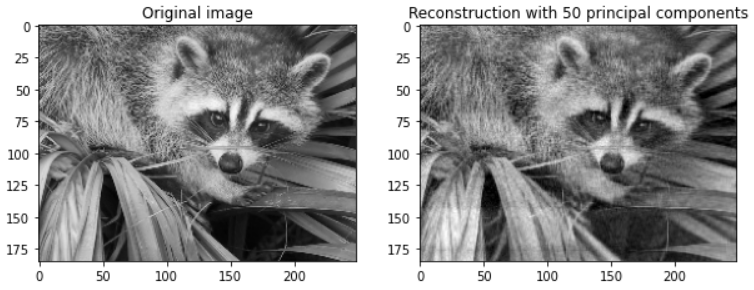
\includegraphics[scale=0.8]{images/racoon_reconstr_50.png}}
    \vfill
    \subfloat[b]{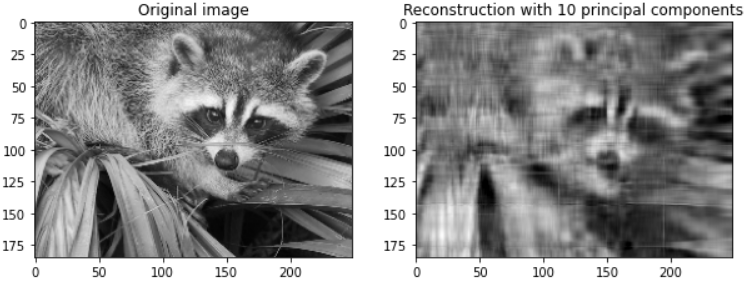
\includegraphics[scale=0.8]{images/racoon_reconstr_10.png}}
    \caption{Different reconstructions of the same image using respectively (a) all, (b) 120, (c) 50, and (d) 10 principal components.}
    \label{fig:racoon-recontrs}
\end{figure}

\paragraph{Part 3}
This part was about applying PCA to data containing trajectories of various pedestrians in the 2D space.
These can be observed in \hyperref[fig:plot-traj]{Figure \ref{fig:trajs}} and it is possible to notice that they are very "fuzzy", probably indicating some amount of noise in the data.\\
Later, we projected the data into the first 2 principal components by computing the SVD decomposition, setting all the singular values after the second one ($\sigma_2$) to zero and reconstructing the projected data through Eq. \ref{eq:svd-reconstr-2}

\begin{equation}\label{eq:svd-reconstr-2}
    \Tilde{X} = US_2V^T
\end{equation}

where $S_2$ is the matrix $S$ coming out of the SVD ($X=USV^T$) where only the first 2 singular values are not set to zero.\\
The first 2 principal components capture 84.92\% of the energy, while to capture most of it ($\geq 90\%$) 3 principal components are necessary.
With 3 principal components it is possible to retain 99.71\% of the energy, which not only suffices to capture most of the dataset's energy (defined as $\geq 90\%$), but it produces an improvement of 14.79\% compared to using 2 principal components.
It is interesting to notice how the behaviour of the first pedestrian (blue) in \textbf{\hyperref[fig:trajs]{Figure \ref{fig:trajs}}(a)} is well represented by the first PCA (also blue) in \textbf{\hyperref[fig:trajs]{Figure \ref{fig:trajs}(b)}}.

\begin{figure}[H]
    \centering
    \subfloat[a]{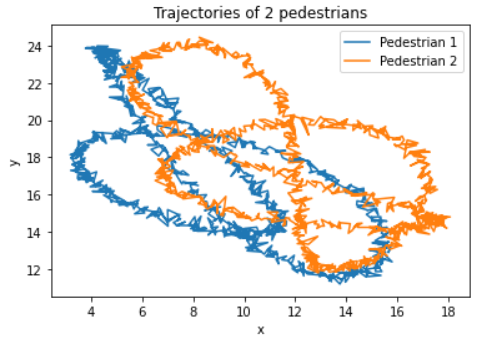
\includegraphics[scale=0.7]{images/trajectories.png}}
    \hfill
    \subfloat[b]{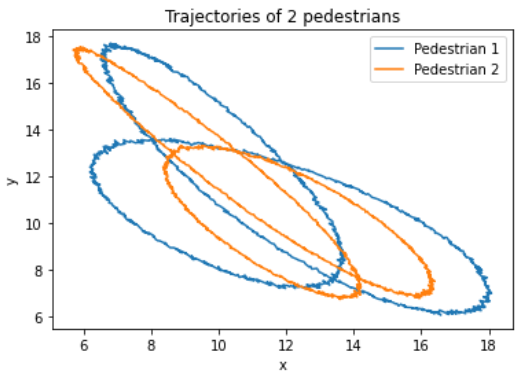
\includegraphics[scale=0.7]{images/pca_2_comps.png}}
    \caption{(a) Trajectories of 2 pedestrians in the 2D space.
    (b) 2 principal components of the 30 dim space.}
    \label{fig:trajs}
\end{figure}

\end{task}

\begin{task}{2, Diffusion Maps}
We implemented most utilities for plotting and computation for this task in a class (\texttt{DiffusionMap}), especially the \texttt{execute\_algorithm} function, corresponding to the algorithm requested by the exercise sheet. The implementation was slightly more difficult to implement with respect to the PCA, with the implementation and testing window being three days due to subtle erroneous mathematical computations due to wrong use of \texttt{numpy} methods. For example we used \texttt{np.linalg.eig} instead of \texttt{np.linalg.eigh} to calculate eigenvalues and eigenvectors, even though at that point the matrix on which actuate the eigendecomposition is Hermitian.\\
To assure the accuracy of measurements, once the procedure proved to be correct, was ensured by the numerical stability of using \texttt{numpy}. The correctness of results was ensured by comparing results with a standard library as \texttt{DataFold} as well as using its measuring utility for backing up our assertions (e.g. using \textit{LocalRegressionSelection} to enforce the correct selection of eigenfunctions for part three of the task.
\paragraph{Part 1}

\begin{figure}[H]
    \centering
    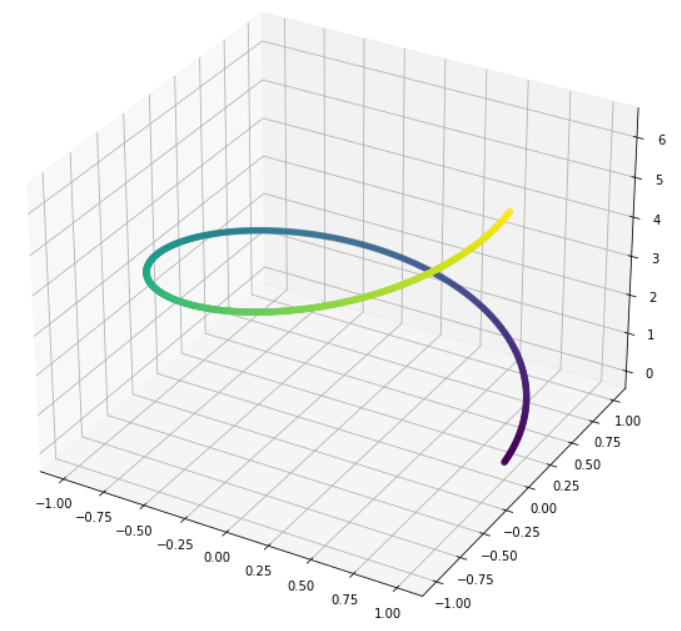
\includegraphics[scale=0.4]{images/task2_1_data.png}
    \caption{dataset of 1000 point, through \texttt{get_part_one_dataset}}
    \label{fig:task-2-1-data}
\end{figure}

The dataset (\textbf{\hyperref[fig:task-2-1-data]{Figure \ref{fig:task-2-1-data}}}) composed of 1000 points is created through a simple implemented method, \texttt{get\_part\_one\_dataset}, and the five (six for a better figure) eigenfunctions $\phi_l$ associated to the largest eigenvalues $\lambda_l$ are shown in \textbf{\hyperref[fig:task1]{Figure \ref{fig:task1}}} against the $t_k$ variable, as requested.

\begin{figure}[h]
\centering
\begin{tabular}{c c c}
\subfloat[a] { 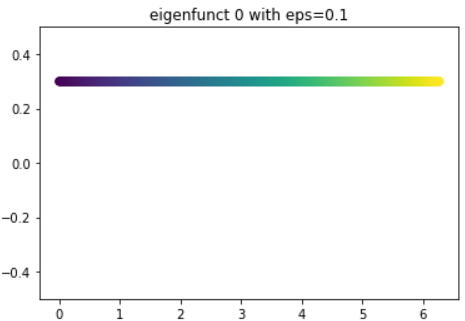
\includegraphics[scale=0.4]{images/task2_1_eig0.png} }
&
\subfloat[b] { 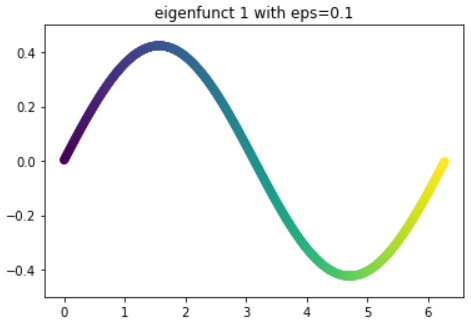
\includegraphics[scale=0.4]{images/task2_1_eig1.png} }
&
\subfloat[c] { 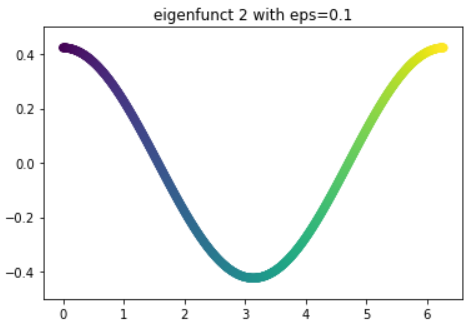
\includegraphics[scale=0.4]{images/task2_1_eig2.png} }
\\
\subfloat[d] { 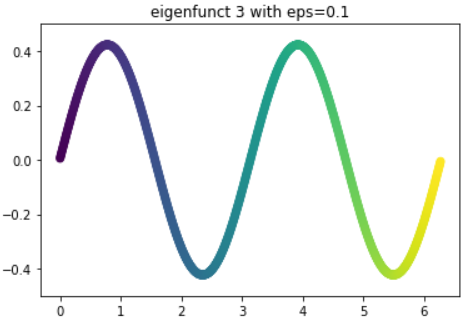
\includegraphics[scale=0.4]{images/task2_1_eig3.png} }
&
\subfloat[e] { 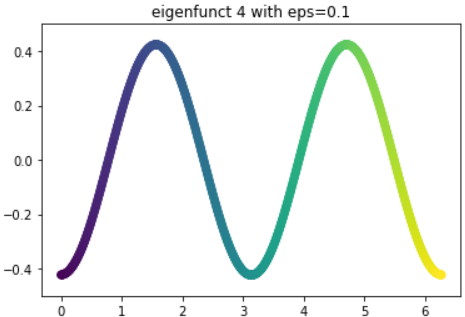
\includegraphics[scale=0.4]{images/task2_1_eig4.png} }
&
\subfloat[f] { 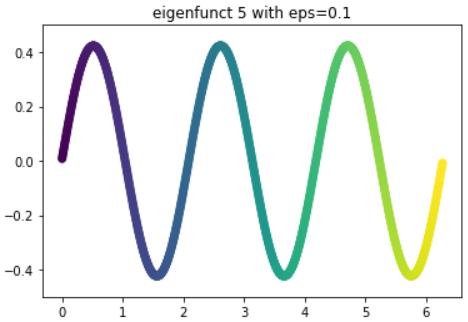
\includegraphics[scale=0.4]{images/task2_1_eig5.png} }
\end{tabular}
\caption{eigenfunctions relative to largest eigenvalues plotted against $t_k$}
\label{fig:task1}
\end{figure}

From the figure can be noticed that the most relevant eigenfunction, (a), is constant. This fact is present also in further figures and is remarked also in the exercise sheet. Another interesting fact is that all eigenfunctions have a sinusoidal behaviour in time, with a higher (f) or lower frequency (b), hinting at the correlation that exists between \textit{Diffusion Maps} and \textit{Fourier Analysis}. Both the methods do in this case in fact portray the original dataset through a combination of sinusoidal waves, with different coefficients and frequency, represented differently in Fourier and in the DM. 

\paragraph{Part 2}
This part of the task focused on using the algorithm to obtain the first ten eigenfunctions of the \textit{Laplace Beltrami} operator on the \textit{swiss roll} manifold. In particular, using \texttt{SkLearn}, the dataset was created with ease, composed of 5000 non-noisy samples as shown in \textbf{\hyperref[fig:swiss-data]{Figure \ref{fig:swiss-data}}}.

The computation of the algorithm retrieves the ten desired eigenfunctions, which are shown (plotted against the first non constant eigenfunction $\phi_1$) in \textbf{\hyperref[fig:swiss5k]{Figure \ref{fig:swiss5k}}}, on which a brief discussion can be applied. First of all it can once again be noticed how $\phi_0$ is constant, as when plotted against $\phi_1$ it delivers a line. Secondly, many other eigenfunctions look to be related to $\phi_1$ as they are in fact functions of it. Examples are $\phi_2$, $\phi_3$ and $\phi_4$. On the contrary the first $\phi$ to deliver a non-function behaviour when plotted agains $\phi_1$ is $\phi_5$. The pairing of $\phi_1$ and $\phi_5$ is a good example (and the first $l>1$ to deliver that!) for a \textit{functional independence}. Finding functional independence in such a \textit{manifold learning model} is fundamental to have non poor embeddings. In fact \textit{functional dependence} means that the first eigenvector $\phi_x$ does not go along a new and independent direction compared to eigenvector $\phi_y$, not giving as much information as could be possibly given in the same dimensional subspace but with a different pair. We further ensured the possibility for ($\phi_1$,$\phi_5$) being a good unfolding is confirmed visually by the figure and mathematically through the use of \textit{LocalRegressionSelection}, a technique available for the selection of most relevant couples, triples, etc (you decide the dimensionality!) of eigenfunctions in data (\textbf{\hyperref[fig:datafold-code]{Figure \ref{fig:datafold-code}}}).

\begin{figure}[h]
\centering
\begin{tabular}{c c}
\subfloat[a] { 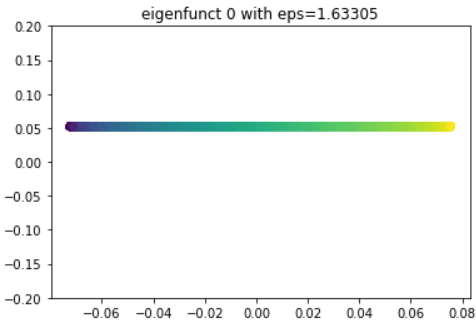
\includegraphics[scale=0.4]{images/sw_5k_eig0.png} }
&
\subfloat[b] { 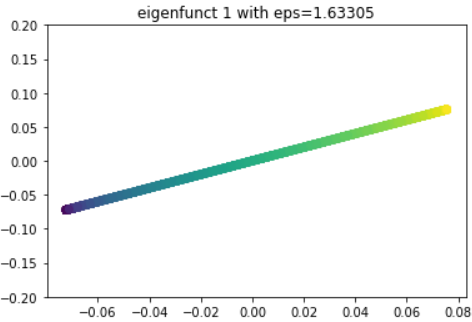
\includegraphics[scale=0.4]{images/sw_5k_eig1.png} }
\\
\subfloat[c] { 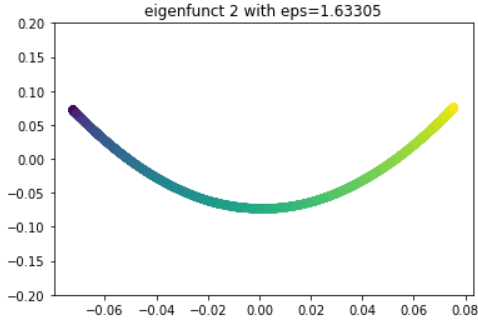
\includegraphics[scale=0.4]{images/sw_5k_eig2.png} }
&
\subfloat[d] { 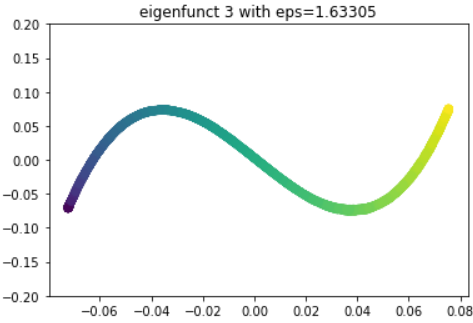
\includegraphics[scale=0.4]{images/sw_5k_eig3.png} }
\\
\subfloat[e] { 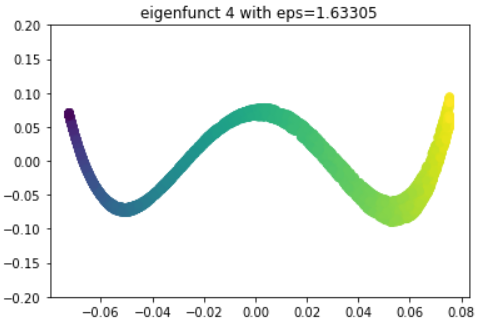
\includegraphics[scale=0.4]{images/sw_5k_eig4.png} }
&
\subfloat[f] { 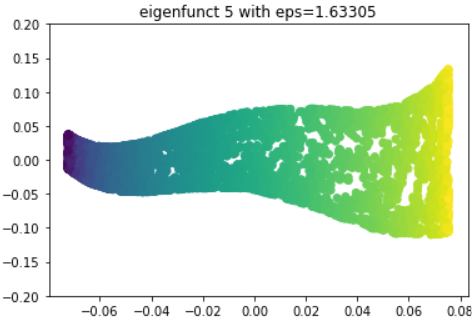
\includegraphics[scale=0.4]{images/sw_5k_eig5.png} }
\\
\subfloat[g] { 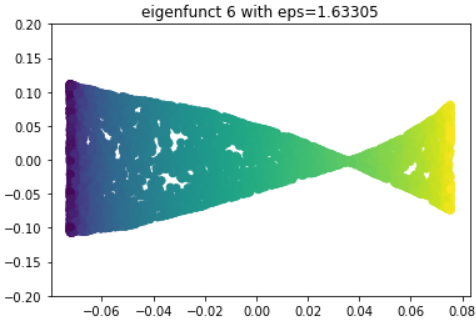
\includegraphics[scale=0.4]{images/sw_5k_eig6.png} }
&
\subfloat[h] { 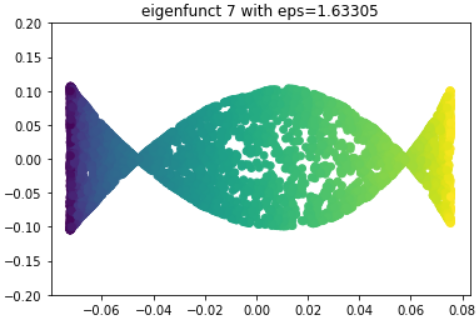
\includegraphics[scale=0.4]{images/sw_5k_eig7.png} }
\\
\subfloat[i] { 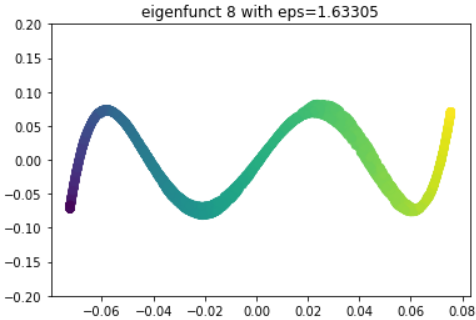
\includegraphics[scale=0.4]{images/sw_5k_eig8.png} }
&
\subfloat[j] { 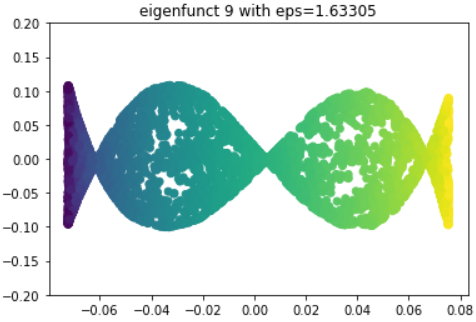
\includegraphics[scale=0.4]{images/sw_5k_eig9.png} }
\\
\end{tabular}
\caption{plots where the first non costant eigenfunction ($\phi_1$) is plotted against the rest (5000 samples)}
\label{fig:swiss5k}
\end{figure}

\begin{figure}[h]
\hspace*{-2cm}
\centering
\begin{tabular}{c c c}
\subfloat[a] { 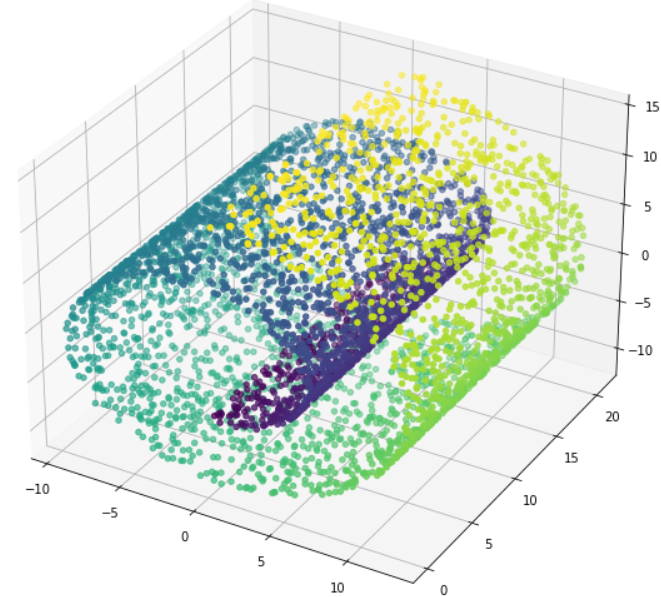
\includegraphics[scale=0.4]{images/sr3d_5000.png} }
&
\subfloat[b] { 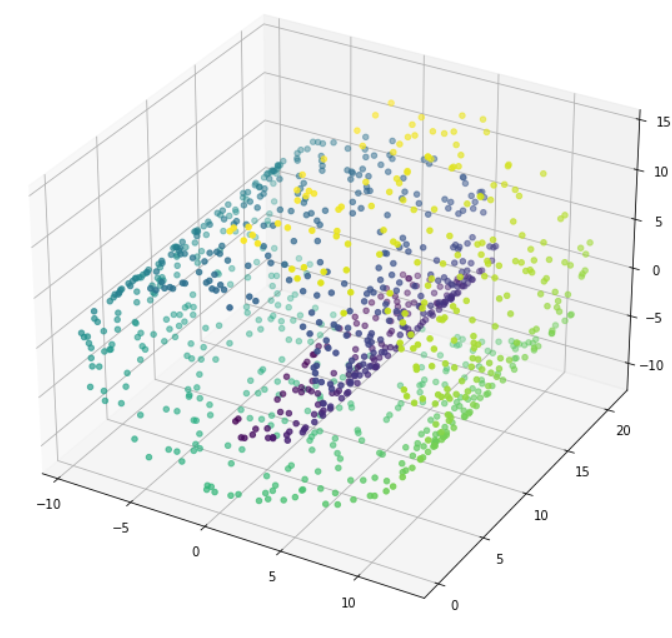
\includegraphics[scale=0.4]{images/sr3d_1000.png} }
&
\subfloat[c] { 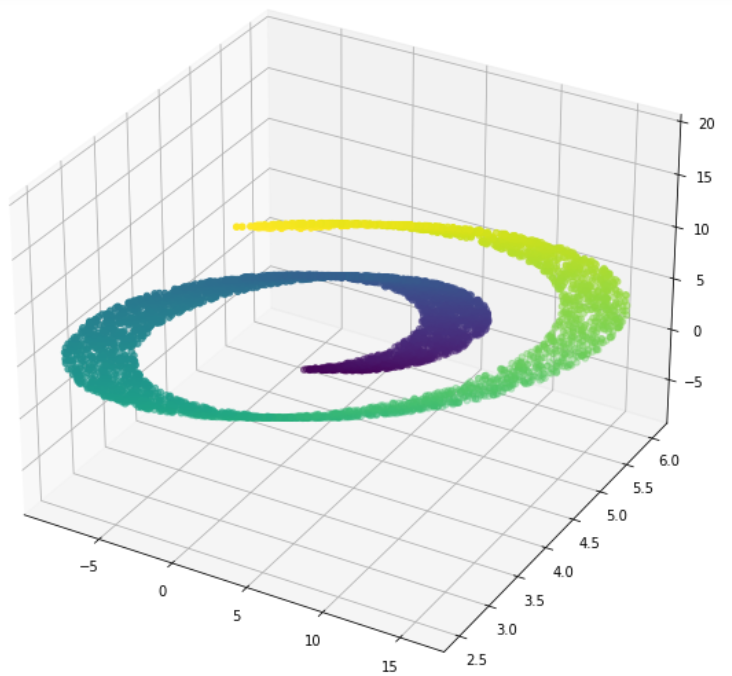
\includegraphics[scale=0.4]{images/sr2d_5000.png} }
\\
\end{tabular}
\caption{swiss roll dataset sampled through \texttt{sklearn} (5000 samples - 1000 samples - only 2 PCA)}
\label{fig:swiss-data}
\end{figure}
\pagebreak

The task proceeds asking to compute the three principal
components of the swiss-roll dataset, which energy result to be, taking away one PC at a time from left to right:
\begin{center}
    \textbf{(1.0, 0.7104704462758858, 0.3933604936493569)}
\end{center}
This already hints at answering the question: \textit{Why is it impossible to only use two principal components to represent
the data?} As one can appreciate both by the \textit{energy value} of using only the first two components as well as looking at the reconstruction proposed by the first two components (\textbf{\hyperref[fig:swiss-data]{Figure \ref{fig:swiss-data}(c)}}), the loss in energy (and therefore data variance) due to not using the third principal component is unbearable for the original data, which looses too much information.

Another interesting proposed experiment involves the number of samples, reducing it from 5000 to 1000 leads to the dataset proposed in \textbf{\hyperref[fig:swiss-data]{Figure \ref{fig:swiss-data}(b)}}. This new dataset is for sure less representative of the manifold with respect to the richer dataset proposed before. The effect of this sparseness travels to the produced \textit{Diffusion Maps}, as can be appreciated in \textbf{\hyperref[fig:swiss1k]{Figure \ref{fig:swiss1k}}}, where the eigenfunctions become much more noisier with respect to the more populated case.

\begin{figure}[h]
\centering
\begin{tabular}{c c c}
\subfloat[a] { 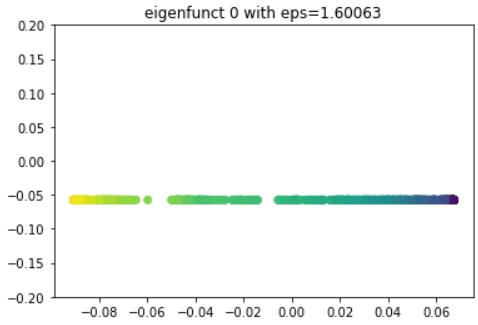
\includegraphics[scale=0.4]{images/sw_1k_eig0.png} }
&
\subfloat[d] { 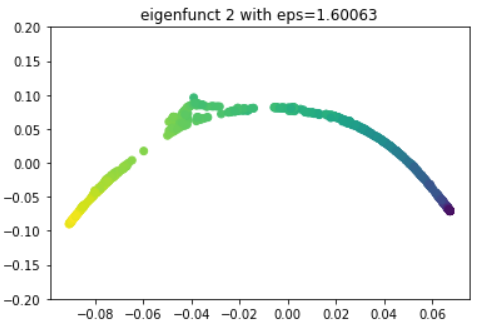
\includegraphics[scale=0.4]{images/sw_1k_eig2.png} }
&
\subfloat[d] { 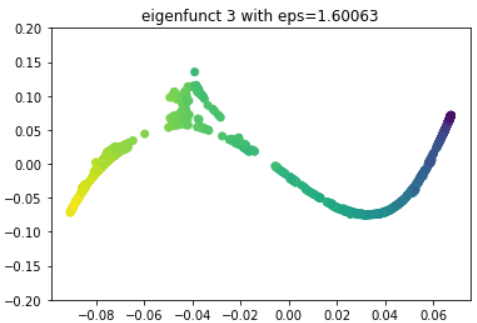
\includegraphics[scale=0.4]{images/sw_1k_eig3.png} }
\\
\subfloat[e] { 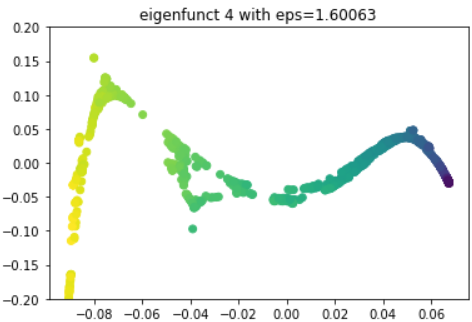
\includegraphics[scale=0.4]{images/sw_1k_eig4.png} }
&
\subfloat[f] { 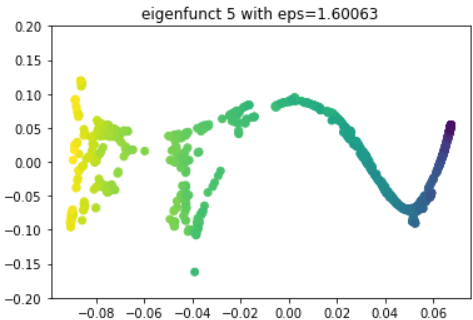
\includegraphics[scale=0.4]{images/sw_1k_eig5.png} }
&
\subfloat[g] { 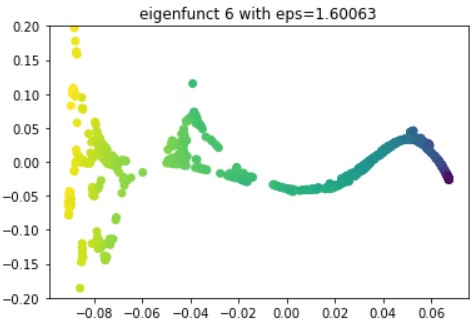
\includegraphics[scale=0.4]{images/sw_1k_eig6.png} }
\\
\subfloat[h] { 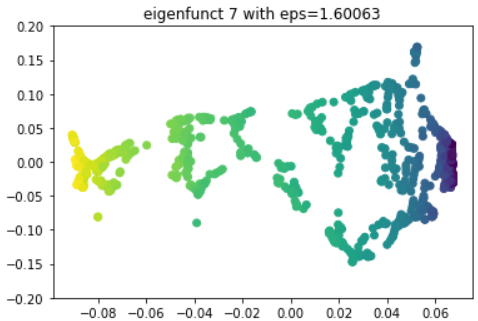
\includegraphics[scale=0.4]{images/sw_1k_eig7.png} }
&
\subfloat[i] { 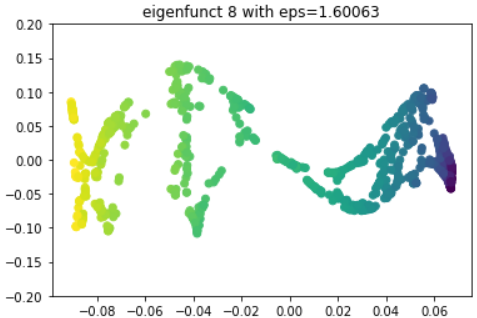
\includegraphics[scale=0.4]{images/sw_1k_eig8.png} }
&
\subfloat[j] { 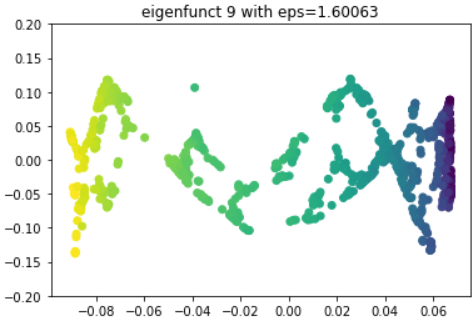
\includegraphics[scale=0.4]{images/sw_1k_eig9.png} }
\\
\end{tabular}
\caption{plots where the first non costant eigenvalue ($\phi_1$) is plotted against the rest (1000 samples)}
\label{fig:swiss1k}
\end{figure}

\paragraph{Part 3}
The final part of this task goes back to a dataset already utilized in \textbf{Task 1}, regarding walking pedestrians (\textbf{\hyperref[fig:trajs]{Figure \ref{fig:trajs}}}). With \textit{Diffusion Maps} it is not possible to use the same concept of energy as previously used with PCA, therefore it helps to first go through a visual route hoping to find a good combination of eigenfunctions. But what is a good combination of eigenfunctions? It is a set of eigenfunctions leading to a subspace where the data is unfolded, meaning there are \textbf{no intersections}. We started taking a look at 3D subspaces with three consecutive eigenfunctions, more for fun than for science rigorosity. 

\begin{figure}[h]
\centering
\begin{tabular}{c c}
\subfloat{ 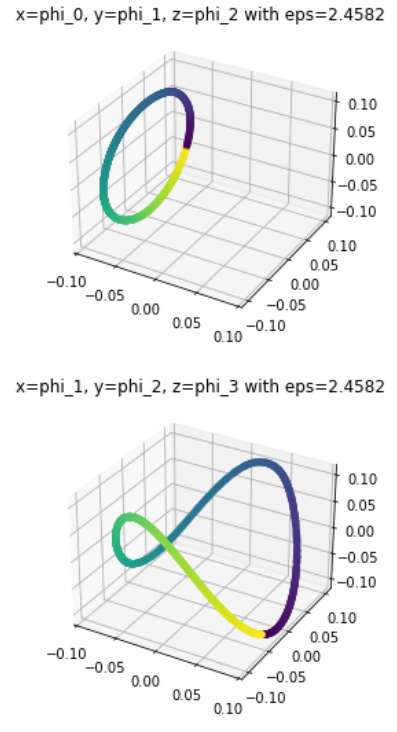
\includegraphics[scale=0.6]{images/ped_3d_0.png} }
&
\subfloat{ 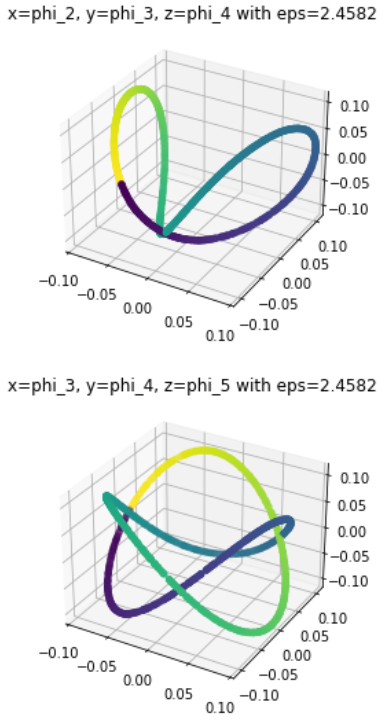
\includegraphics[scale=0.6]{images/ped_3d_1.png} }

\end{tabular}
\caption{example of 3 consecutive eigenfunctions (showing possibility of no intersection)}
\label{fig:ped-3d}
\end{figure}
The result shown in \textbf{\hyperref[fig:ped-3d]{Figure \ref{fig:ped-3d}}} shows that in the 3D space it is possible to fully unfold the data (for example look at the subspace defined by $\phi_1$, $\phi_2$, $\phi_3$) but that no all combinations are unfolding the data (for example $\phi_2$, $\phi_3$, $\phi_4$). An interesting triple is the first one, where the usual $\phi_0$ being constant shows how there can possibly be a 2D subspace already showing a good combination of eigenfunctions.

\begin{figure}[h]
\centering
\begin{tabular}{c c}
\subfloat{ 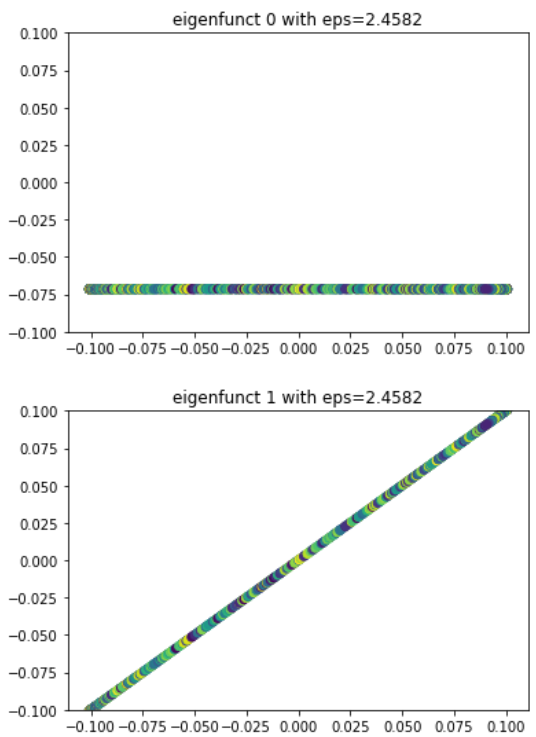
\includegraphics[scale=0.4]{images/ped_2d_0.png} }
&
\subfloat{ 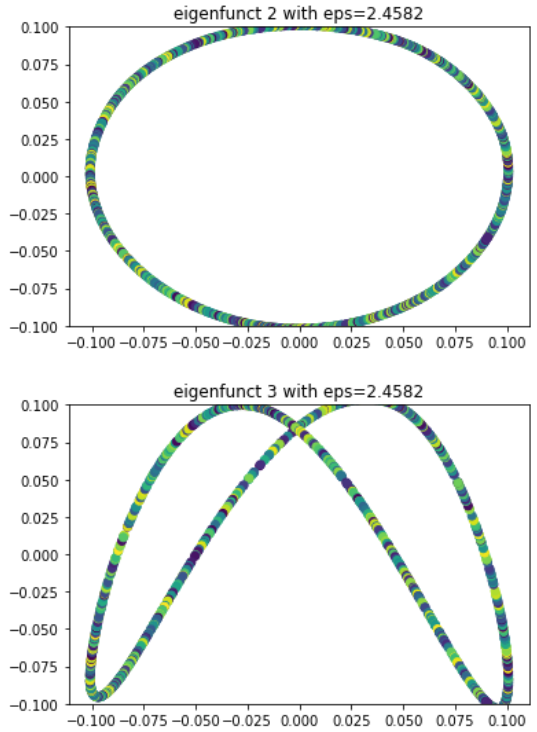
\includegraphics[scale=0.4]{images/ped_2d_1.png} }
\\
\subfloat{ 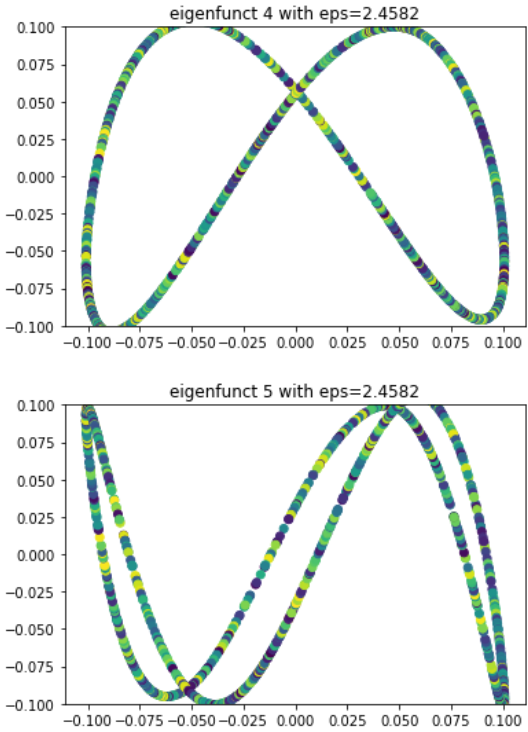
\includegraphics[scale=0.4]{images/ped_3d_2.png} }
&
\subfloat{ 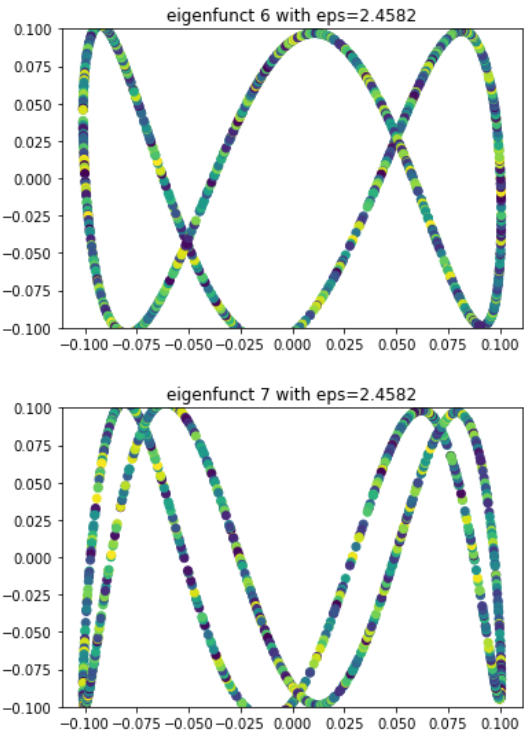
\includegraphics[scale=0.4]{images/ped_3d_3.png} }

\end{tabular}
\caption{2D latent space of eigenfunctions, first one is always $\phi_1$ (showing possibility of no intersection in 2D)}
\label{fig:ped-2d}
\end{figure}
Eventually the test was moved to searching in 2D subspaces, as shown in \textbf{\hyperref[fig:ped-2d]{Figure \ref{fig:ped-2d}}}. The hint given by the 3D plots was confirmed, showing how the subspace produced by $\phi_1$ and $\phi_2$ has no intersections and is therefore a \textit{proper embedding}. Knowing that the 2D space can have a good embedding led us to confirm our findings by utilizing again \textit{LocalRegressionSelection}, which as can be seen in \textbf{\hyperref[fig:ped-code]{Figure \ref{fig:ped-code}}}, retrieves the same results.

\begin{figure}[H]
    \centering
    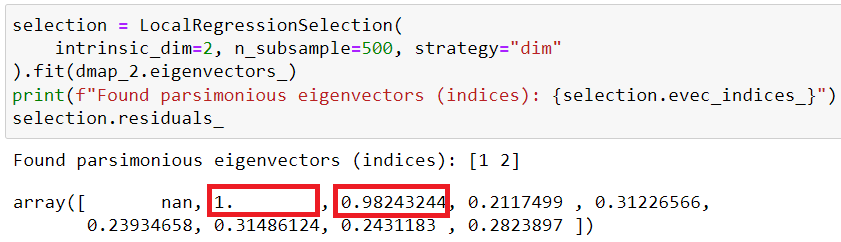
\includegraphics[scale=0.7]{images/ped_choose.png}
    \caption{code showing a possible selection modality}
    \label{fig:ped-code}
\end{figure}

\pagebreak 
\paragraph{Bonus}
After having downloaded \textit{DataFold} library on Windows, we followed the tutorial already present for the \textit{s-curve manifold} and changed the necessary bits to apply the same snippet on the \textit{swiss-roll manifold}. The code proved to be very easy and intuitive as well as being optimized and therefore reasonably fast. Much compact and we would for sure recommend it for this case scenario. Plotting the \textit{swiss-roll} eigenfunctions brings the same results produced by our implementation, as can be appreciated in \textbf{\hyperref[fig:datafold-swiss]{Figure \ref{fig:datafold-swiss}}}. The incredibly useful part of having delved into this library is finding how actually is possible to understand which are the most relevant eigenfunctions for a good reduction and therefore a good embedding. In fact, having a 2D, 3D or 4D space makes it still reasonable to find good eigenfunction combination with our bare eyes, but in higher space the situation is much more complicated. A possible solution to that is given by the library, utilizing (mentioning here for the third time!) \textit{LocalRegressionSelection}, which gives the relevance of each eigenfunction given a precise dimensionality reduction (\textbf{\hyperref[fig:datafold-code]{Figure \ref{fig:datafold-code}}}).

\begin{figure}[H]
    \centering
    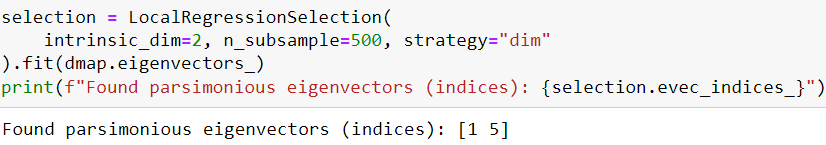
\includegraphics[scale=0.7]{images/datafold-code.png}
    \caption{code showing an automatic selection of the best choice pair $\phi_l$ (with a given dimension)}
    \label{fig:datafold-code}
\end{figure}

\pagebreak
\begin{figure}[H]
    \centering
    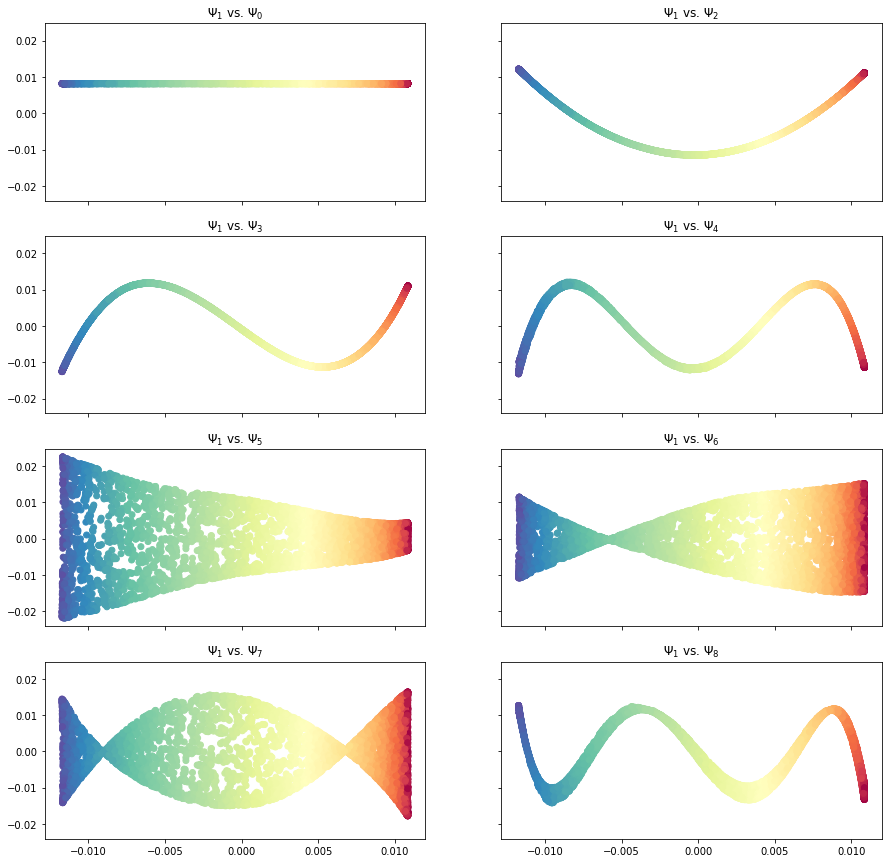
\includegraphics[scale=0.4]{images/datafold_swiss_roll.png}
    \caption{$\phi_1$ against the other eigenfunctions using datafold - swiss roll}
    \label{fig:datafold-swiss}
\end{figure}

\end{task}


\begin{task}{3, Variational Autoencoders}
This task proved to be the most time consuming due to library set up issues, with the implementation and testing taking six to seven days. The implementation started by attempting to implement the code proposed by the tutorial mentioned in the exercise sheet. A first problem came up with the \texttt{TensorFlow} version required, since our laptops had \texttt{TensorFlow 2.7.0} installed. After setting up a virtual environment with the version 1.15 (which also requires a Python version below 3.8, leading to other setting up annoying situations), we started playing with the model, seeing the functioning of it. We were not anyway fully satisfied with this implementation, therefore, being masochists, we moved to \texttt{TensorFlow 2}, a useful experience to understand some of the main differences between the two major releases. Eventually we decided to go to \texttt{Pytorch} (version 1.9.0 with Python 3.8.6), where we remained to implement our final solution. \\After the rollercoaster of libraries we decided to implement the model in a class (\texttt{VAE}) subclassing \texttt{nn.Module}, containing some fundamental methods and the required globally trainable variable defining the reconstruction \textit{standard deviation}:
\begin{itemize}
    \item \texttt{\_\_init\_\_}: initializer, allows to give the input data dimensionality, as well as the feature space dimensionality (number of neurons in hidden layers) and finally the latent space dimensionality (both for the \textit{mean} and the \textit{scale}). Batch size is always excluded from these dimensions. An additional parameter has been added (\texttt{use\_BCE\_loss}) to allow for a quick change in behaviour of last decoder activation function, switching from \textit{sigmoid} to \textit{linear}. This will be further discussed later.
    \item \texttt{reparameterize}: applies the reparameterization trick to allow backprop to flow to encoder part of the model
    \item \texttt{encode}: applies feedforward to the encoder model, getting as input the data from the dataloader and outputting the \textit{mean} and \textit{log variance} of the latent space distribution. We decided to output the \textit{log variance} for convenience in the \textit{KLDivergence} loss. We anyway reverted it back to the \textit{standard deviation} where needed (e.g. in the reparameterization trick)
    \item \texttt{decode}: applies the feedforward to the decoder model, getting as input data sample batch from the latent space and outputting the \textit{mean} of the output distribution
    \item \texttt{forward}: applies the overall feedforward, calling the encode and decode method internally, outputting both the means and the log variance (only the one coming from the latent space)
    \item \texttt{generate\_many}: utility function to call decode multiple times after having sampled data from the latent space the same number of times
    \item \texttt{log\_var\_rec}: an \texttt{nn.Parameter}, implementing the globally trainable \textit{standard deviation} for the reconstruction distribution. Actually, once again, we are treating this variable as the \textit{log variance} for the alternative loss (will be introduced later) convenience. This does not hinder the possibility of retrieving the \textit{standard deviation} where needed by applying some exponential transformation.
\end{itemize}

The other utilities needed for training and plotting have been relegated to \texttt{vae\_utils.py}, which contains in particular utilities for:
\begin{itemize}
    \item fitting the model
    \item testing the model
    \item calculating the ELBO loss
    \item plotting/saving the \textbf{15} reconstructed digits with respect to the input data
    \item plotting/saving the produced latent space over the test dataset
    \item plotting/saving the produced latent space over the test dataset, but using digits and not scatter (see Figureasd)
    \item plotting/saving the \textbf{15} generated digits sampled from the latent space
\end{itemize}

A peculiarity that can be found is that we decided to propose two alternatives in the training, varying the \textit{reconstructed loss}. This was also the reason for several time spent over implementation and \textbf{research}, as having the mean as output is not taken in consideration by a large part of the implementations out there. Going more in detail:
\begin{itemize}
    \item the \textit{standard} training/testing method: we implemented the reconstruction loss utilizing \texttt{BCELoss}, a Cross Entropy solution which has as general objective finding the difference between two probability distributions, in our case the output distribution and the input distribution. The reconstruction loss is therefore computed by the library and is added to the KLD.
    \item the \textit{alternative} training/testing method: we decided to also implement a loss which could take advantage of the globally trained log variance as well as being more faithful to the ELBO definition. We therefore mathematically hardcoded the definition of \textit{log likelihood} of  a sample (input data in our case) given the output distribution (which is supposed to be a normal distribution).
\end{itemize}

\begin{figure}[H]
    \centering
    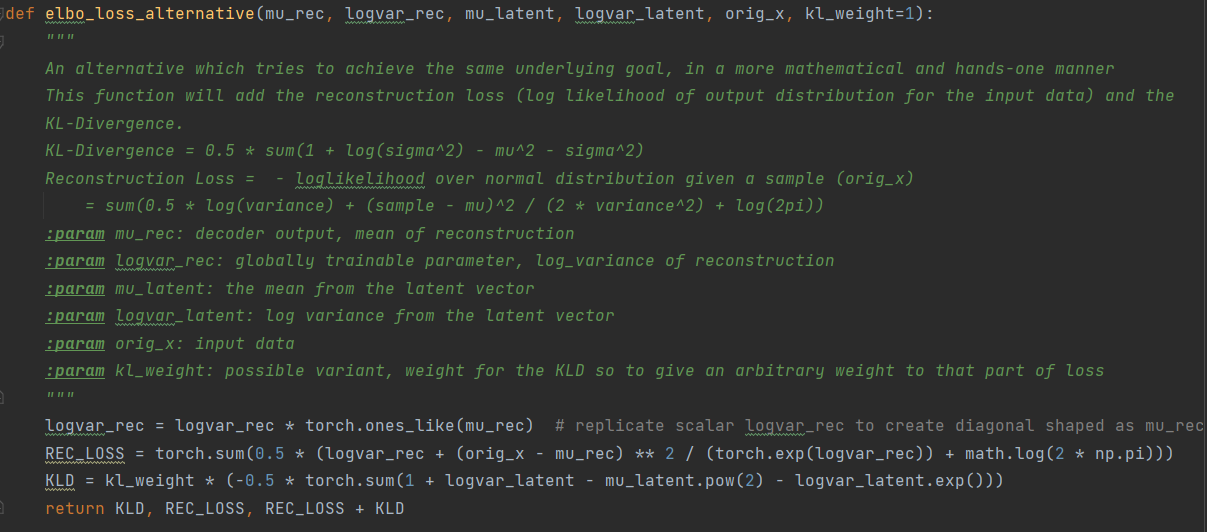
\includegraphics[scale=0.6]{images/elbo_alt.png}
    \caption{elbo loss utilized for the \textit{alternative} implementation}
    \label{fig:alt-elbo}
\end{figure}
Changing from \textit{standard} to \textit{alternative} can be simply achieved by swapping between using methods \textit{fit/fit\_alternative} and \textit{test/test\_alternative}.
After this brief discussion the usefulness of the aforementioned \texttt{use\_BCE\_loss} parameter might become clearer. The \textit{standard} implementation needs a sigmoid as last decoding activation function since the output is expected to be between 0 and 1, while the \textit{alternative} does not. That parameter easily allows for the presence or absence of said activation function. 

\paragraph{Part 1}
The first part of the task asks for two reasoning questions:
\begin{itemize}
    \item \textit{What activation functions should be used for the mean and standard deviation of the approximate posterior
and the likelihood|and why?}: since the probability distributions we want to follow are multivariate gaussian distribution we should avoid \textit{mean} and \textit{standard deviation} values which are not valid for modelling such a distribution. A multivariate gaussian distribution is in particular parametrized with a \textit{real mean} and a \textit{positive standard deviation} in matrix form (positive semi-definite matrix in particular). Therefore there should be no constraint on the \textit{mean} as it can take whatever real value. Regarding the \textit{standard deviation} instead, since it has to be formed of positive values, there should be some care in utilizing a non-negative (but with no upper limit) activation function, such as ReLU or Softplus. As a little parenthesis, in our case this problem is not present, as utilizing the \textit{log variance} leads to the possibility of having negative values (so no need for activation functions) while the constraint of a positive \textit{standard deviation} is maintained per se.
    \item \textit{What might be the reason if we obtain good reconstructed but bad generated digits?}: having good generated digits all depend on having a good latent space. If the latent space discriminates well between classes and is well distributed (while not being too sparse) then the results will be fantastic, with coherence in near points. Problems and therefore bad generations can appear for a number of reasons in VAE. First of all it might be the case that the net is \textit{not powerful enough}, but this would also mean that not only the generated but also the reconstructed images are not the best. Secondly, there could be an \textit{imbalance} between the two addends of the KL Divergence, leading to other approaches such as $\beta$-VAE where the two addends get weighted. If KL Divergence is irrelevant then the VAE is pretty much a basic AE, with more effort in learning a mapping than an actual space reduction. Lastly, the problem could be related to having a \textit{too high dimensional latent space}. That is also the case in our scenario when going from 2 to 32 dimensions in the latent space. In fact if your latent space is too big, it can lead to generating out-of-distribution samples because the latent space gets incredibly sparse. This can lead to seeing sharp blobs of white and black, or maybe seeing the same digit over and over. If we were to take this concept to the extreme we could actually reach an \textit{overfitted latent space}, where the dimensionality of the latent space is equal to the number of training data, with each training data being mapped in the latent space to a different and orthogonal dimension.
\end{itemize}

\paragraph{Part 2}
This second part is centered on showing the results of training a VAE model with some given hyperparameters on the MNIST dataset. The dataset is normalized between 0 and 1, dividing each cell by 255 (the image is a single channel grayscale). We are going to first show the results on the \textit{standard} implementation to then move to the \textit{alternative}.

\pagebreak\textbf{\hyperref[fig:vae-code]{Figure \ref{fig:vae-code}}} reports the model implementation of the most important methods:
\begin{figure}[h!]\centering
\subfloat{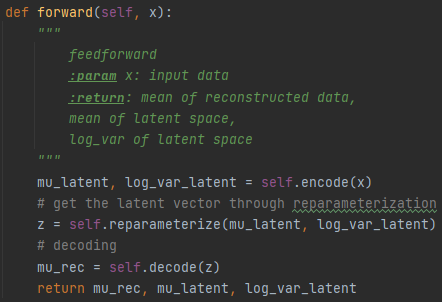
\includegraphics[width=.35\linewidth]{images/forward.png}}\\
\subfloat{\includegraphics[width=.45\linewidth]{images/encode.png}}\\
\subfloat{\includegraphics[width=.55\linewidth]{images/decode.png}}
\caption{main model methods - from top to bottom \textit{forward}, \textit{encode}, \textit{decode} }
\label{fig:vae-code}
\end{figure}

\textit{Standard} results for loss and the required plots about latent space, reconstruction and generation are shown in \textbf{\hyperref[fig:loss-standard]{Figure \ref{fig:loss-standard}}} (losses), \textbf{\hyperref[tab:bce2d]{Figure \ref{tab:bce2d}}} (results 2D latent space) and  \textbf{\hyperref[tab:bce32d]{Figure \ref{tab:bce32d}}} (results 32D latent space). Analyzing the images some interesting discussion can be brought up. In the loss figure it is possible to see that both in the case of 2D and 32D latent space, as the reconstruction loss gets lower and lower (the model is learning well how to reconstruct the input images), the KL Divergence rises to act as a \textit{regularizer}. This gives the desired effect, with the model being slightly less perfect in reconstructing if put in comparison with a normal \textit{AutoEncoder} to fulfill the objective of creating a meaningful latent space. 

Continuing the analysis on the 2D case, \textbf{\hyperref[tab:bce2d]{Figure \ref{tab:bce2d}}} shows the results divided by epoch. In particular it is possible to appreciate the evolution of the latent space, which in the end is a 2D distribution that maintains coherence between nearby points, effectively dividing the classification in space regions. Taking instead a look at the reconstruction it is possible to notice how the data (first row of each plot) gets reconstructed better and better as epochs go on, as is also deductible by the decreasing \textit{loss}. The VAE model gets better at reconstructing while also constructing a relevant latent space, from which generated samples become more and more trustworthy, as can be noticed in the same figure. The generated images look a little blurry but for sure readable.

Comparing the just discussed results with the results portrayed in \textbf{\hyperref[tab:bce32d]{Figure \ref{tab:bce2d}}}, one can reassert what already expressed in \textbf{Part 1} of this task. The reconstructed images do in fact look much better, appearing almost identical to the original data by the end of the training. This happens because the latent space is much bigger than before, allowing for a clearer internal representation of the data, nevertheless hindering the generation capability. The sharpness in reconstructing is in fact transferred to the generation capability, where the generated images are much sharper but less understandable. One can in fact appreciate in the last pictured epochs how some numbers are not at all understandable, probably due once again to the higher dimensional latent space which leads to a sparser data representation. It is interesting to notice how the KL Divergence grows much higher with respect to the 2D case, trying to regularize a bigger latent space, effectively creating a bigger gap between the \textit{total loss} and the \textit{reconstruction loss}.

Briefly moving on to the \textit{alternative} implementation, the results for loss and the required plots about latent space, reconstruction and generation are shown in \textbf{\hyperref[fig:loss-alternative]{Figure \ref{fig:loss-alternative}}} (losses), \textbf{\hyperref[loglike2d]{Figure \ref{tab:loglike2d}}} (results 2D latent space) and  \textbf{\hyperref[tab:loglike32d]{Figure \ref{tab:loglike32d}}} (results 32D latent space). The loss behaviour is similar to the models using \textit{Cross Entropy}, with a little slower loss/KL Divergence descent/ascent. One might notice that the loss reaches a negative value, a peculiar behaviour for sure. This can be explained by the reconstruction distribution: we monitored the change in value of the globally trainable \textit{log variance} and noticed how it decreased until reaching a negative value (which is possible), meaning the standard deviation of the reconstructed distribution stands between 0 and 1. This leads to a narrow multivariate distribution, for which the log likelihood can possibly give a negative value. The model proved nevertheless to improve its capabilities and could continue to learn, further lowering the loss.

Another interesting difference between \textit{standard} and \textit{alternative} can be instead noticed in the \textit{latent space} construction. Apart from having a rougher start compared to the \textit{standard} implementation, the \textit{alternative} tends to reach a \textit{zero centered} distribution, distinctively different from the other created \textit{latent space} (the experiment has been repeated multiple times, the behaviour stays the same). 
Finally, moving to the generated and reconstructed images, there is no noticeable difference in the 2D aspect, while a relevant decrease in generation capability can be appreciated in the 32D case if compared to the analogous with the \textit{standard} implementation.


\begin{figure}[t]\centering
\subfloat{\includegraphics[width=.4\linewidth]{images/loss.png}} \hspace{1.5cm}
\subfloat{\includegraphics[width=.4\linewidth]{images/l_32_bce/loss.png}}
\caption{total loss and sublosses (KLD and REC) for both the \textit{standard} 2d (left) and 32d (right) latent space}
\label{fig:loss-standard}
\end{figure}
\pagebreak 

% ------------------------------------ %

\begin{figure}\centering
\subfloat{\includegraphics[width=.4\linewidth]{images/l_2/loss.png}} \hspace{1.5cm}
\subfloat{\includegraphics[width=.4\linewidth]{images/l_32/loss.png}}
\caption{total loss and sublosses (KLD and REC) for both the \textit{alternative} 2d (left) and 32d (right) latent space}
\label{fig:loss-alternative}
\end{figure}
\end{task}


\begin{task}{4, Fire Evacuation Planning for the MI Building}
The last task asks for the use of Machine Learning for the analysis of people distribution in the MI Building in the case of need for a fire evacuation. In particular it is interesting to study where people density gets high, so to plan ahead and possibly give different escape routes to different groups. We had little time remaining for this last task, so it took us only a day but at the same time we did not get the results we wanted. Through this task we learned that even little dimensional input datasets can prove to be hard to tackle.

The initial part of the task asks to download the dataset (which is in \texttt{.npy} format). The scatter of both the train and test set  can be appreciated in \textbf{\hyperref[fig:loss-alternative]{Figure \ref{fig:loss-alternative}}}.

\begin{figure}[H]
    \centering
    \includegraphics[scale=0.4]{images/mi_building.png}
    \caption{MI Building dataset train (\textit{left}) and test (\textit{right}), relevant region is the \textit{red rectangle}}
    \label{fig:alt-elbo}
\end{figure}

The training on this data proved that our model is insufficient since it is limited to efficiently learning data distribution that lies between 0 and 1. Unfortunately this dataset proved very sensitive to rescaling, with the suggested $(-1, 1)$ being the only scaling to lead to consistent training. We achieved the scaling with \texttt{SkLearn} method \texttt{MinMaxScaler}, so we could both transform and transform back (to see the reconstruction in the original space) the data. To train the data we changed the input and ouput neurons to being 2 instead of 748.

After trying various changes in activation function and intermediate dimensions the dataset proved to be difficult to fit. This fact, combined with our model suboptimality in representing output distributions, leads to results which are not the best.
The final model we utilized has the following hyperparameters:
\begin{itemize}
    \item \textit{learning rate}: 0.001 
    \item \textit{batch size}: 64
    \item \textit{epochs}: 100
    \item \textit{latent dimensionality}: 10
    \item \textit{intermediate dimensionality}: 512
    \item \textit{number of hidden layers}: 2 for the encoder, 2 for the decoder
\end{itemize}

The resulting model gave the loss plot proposed in \textbf{\hyperref[fig:mi-loss]{Figure \ref{fig:mi-loss}}}, highly unstable as one can appreciate, showing probably the need for a lower learning rate (which we tried!) or a more thorough hyperparameter search (which we did not do due to time constraints, we simply sampled some configurations).  
\begin{figure}[H]
    \centering
    \includegraphics[scale=0.4]{images/loss-mi.png}
    \caption{loss for VAE model trained on the MI Building dataset}
    \label{fig:mi-loss}
\end{figure}

The resulting reconstruction can be seen in \textbf{\hyperref[fig:mi-rec]{Figure \ref{fig:mi-rec}}}, showing that the model has only learnt the entrance behaviour, without being able to capture more subtler events such as the corridors in the building and not even a big event such as the bar! 

\begin{figure}[H]
    \centering
    \includegraphics[scale=0.4]{images/test-rec-mi.png}
    \caption{reconstruction after training on MI Building dataset - test (left) train (right)}
    \label{fig:mi-rec}
\end{figure}

Lastly, to answer the last question, a continuous generation showed that the critical number for the MI building as predicted for our model is pretty little: \textbf{$\sim$1000}. An example of generating 1000 people with the number of people in the red box being underneath the figure is shown in \textbf{\hyperref[fig:mi-gen]{Figure \ref{fig:mi-gen}}}
\begin{figure}[H]
    \centering
    \includegraphics[scale=0.8]{images/generated-mi.png}
    \caption{generation of 1000 people}
    \label{fig:mi-gen}
\end{figure}

\end{task}

\newpage
\bibliographystyle{plain}
\bibliography{Literature}
\section{Figures}


\begin{table}
[h]
  \begin{tabular}{p{0.2\textwidth}p{0.3\textwidth}p{0.3\textwidth}}
  \hline Epoch num & 15 reconstructed & 15 generated\\
      \hline \textbf{Epoch 1} & \parbox[c]{10em}{
      \hfill\includegraphics[width=1.3\linewidth]{images/l_32_bce/output0.png}} & \parbox[c]{10em}{
      \includegraphics[width=1.3\linewidth]{images/l_32_bce/generated0.png}}\\
      \textbf{Epoch 5} & \parbox[c]{10em}{
      \hfill\includegraphics[width=1.3\linewidth]{images/l_32_bce/output4.png}} & \parbox[c]{10em}{
      \includegraphics[width=1.3\linewidth]{images/l_32_bce/generated4.png}}\\
      \textbf{Epoch 25} & \parbox[c]{10em}{
      \hfill\includegraphics[width=1.3\linewidth]{images/l_32_bce/output24.png}} & \parbox[c]{10em}{
      \includegraphics[width=1.3\linewidth]{images/l_32_bce/generated24.png}}\\
      \textbf{Epoch 50} & \parbox[c]{10em}{
      \hfill\includegraphics[width=1.3\linewidth]{images/l_32_bce/output49.png}} & \parbox[c]{10em}{
      \includegraphics[width=1.3\linewidth]{images/l_32_bce/generated49.png}}\\
      \textbf{Epoch 100} & \parbox[c]{10em}{
      \hfill\includegraphics[width=1.3\linewidth]{images/l_32_bce/output99.png}} & \parbox[c]{10em}{
      \includegraphics[width=1.3\linewidth]{images/l_32_bce/generated99.png}}\\
      \hline
  \end{tabular}
  \caption{results for \textit{standard} implementation - \textbf{32D latent space}} \label{tab:bce32d}
\end{table}

\begin{table}
[h]
  \begin{tabular}{p{0.2\textwidth}p{0.3\textwidth}p{0.3\textwidth}}
  \hline Epoch num & 15 reconstructed & 15 generated\\
      \hline \textbf{Epoch 1} & \parbox[c]{10em}{
      \hfill\includegraphics[width=1.3\linewidth]{images/l_32/output0.png}} & \parbox[c]{10em}{
      \includegraphics[width=1.3\linewidth]{images/l_32/generated0.png}}\\
      \textbf{Epoch 5} & \parbox[c]{10em}{
      \hfill\includegraphics[width=1.3\linewidth]{images/l_32/output4.png}} & \parbox[c]{10em}{
      \includegraphics[width=1.3\linewidth]{images/l_32/generated4.png}}\\
      \textbf{Epoch 25} & \parbox[c]{10em}{
      \hfill\includegraphics[width=1.3\linewidth]{images/l_32/output24.png}} & \parbox[c]{10em}{
      \includegraphics[width=1.3\linewidth]{images/l_32/generated24.png}}\\
      \textbf{Epoch 50} & \parbox[c]{10em}{
      \hfill\includegraphics[width=1.3\linewidth]{images/l_32/output49.png}} & \parbox[c]{10em}{
      \includegraphics[width=1.3\linewidth]{images/l_32/generated49.png}}\\
      \textbf{Epoch 100} & \parbox[c]{10em}{
      \hfill\includegraphics[width=1.3\linewidth]{images/l_32/output99.png}} & \parbox[c]{10em}{
      \includegraphics[width=1.3\linewidth]{images/l_32/generated99.png}}\\
      \hline
  \end{tabular}
  \caption{results for \textit{alternative} implementation - \textbf{32D latent space}} \label{tab:loglike32d}
\end{table}

\begin{table}
  \begin{tabular}{p{0.1\textwidth}p{0.3\textwidth}p{0.3\textwidth}p{0.3\textwidth}}
  \hline Epoch num & latent space & 15 reconstructed & 15 generated\\
      \hline \textbf{Epoch 1} & \parbox[c]{10em}{
      \includegraphics[width=1.3\linewidth]{images/latent_space0.png}} & \parbox[c]{10em}{
      \hfill\includegraphics[width=1.3\linewidth]{images/output0.png}} & \parbox[c]{10em}{
      \includegraphics[width=1.3\linewidth]{images/generated0.png}}\\
      \textbf{Epoch 5} & \parbox[c]{10em}{
      \includegraphics[width=1.3\linewidth]{images/latent_space4.png}} & \parbox[c]{10em}{
      \hfill\includegraphics[width=1.3\linewidth]{images/output4.png}} & \parbox[c]{10em}{
      \includegraphics[width=1.3\linewidth]{images/generated4.png}}\\
      \textbf{Epoch 25} & \parbox[c]{10em}{
      \includegraphics[width=1.3\linewidth]{images/latent_space24.png}} & \parbox[c]{10em}{
      \hfill\includegraphics[width=1.3\linewidth]{images/output24.png}} & \parbox[c]{10em}{
      \includegraphics[width=1.3\linewidth]{images/generated24.png}}\\
      \textbf{Epoch 50} & \parbox[c]{10em}{
      \includegraphics[width=1.3\linewidth]{images/latent_space49.png}} & \parbox[c]{10em}{
      \hfill\includegraphics[width=1.3\linewidth]{images/output49.png}} & \parbox[c]{10em}{
      \includegraphics[width=1.3\linewidth]{images/generated49.png}}\\
      \textbf{Epoch 100} & \parbox[c]{10em}{
      \includegraphics[width=1.3\linewidth]{images/latent_space99.png}} & \parbox[c]{10em}{
      \hfill\includegraphics[width=1.3\linewidth]{images/output99.png}} & \parbox[c]{10em}{
      \includegraphics[width=1.3\linewidth]{images/generated99.png}}\\
      \hline
  \end{tabular}
  \caption{results for \textit{standard} implementation - \textbf{2D latent space}} \label{tab:bce2d}
\end{table}


\begin{table}
  \begin{tabular}{p{0.1\textwidth}p{0.3\textwidth}p{0.3\textwidth}p{0.3\textwidth}}
  \hline Epoch num & latent space & 15 reconstructed & 15 generated\\
      \hline \textbf{Epoch 1} & \parbox[c]{10em}{
      \includegraphics[width=1.3\linewidth]{images/l_2/latent_space0.png}} & \parbox[c]{10em}{
      \hfill\includegraphics[width=1.3\linewidth]{images/l_2/output0.png}} & \parbox[c]{10em}{
      \includegraphics[width=1.3\linewidth]{images/l_2/generated0.png}}\\
      \textbf{Epoch 5} & \parbox[c]{10em}{
      \includegraphics[width=1.3\linewidth]{images/l_2/latent_space4.png}} & \parbox[c]{10em}{
      \hfill\includegraphics[width=1.3\linewidth]{images/l_2/output4.png}} & \parbox[c]{10em}{
      \includegraphics[width=1.3\linewidth]{images/l_2/generated4.png}}\\
      \textbf{Epoch 25} & \parbox[c]{10em}{
      \includegraphics[width=1.3\linewidth]{images/l_2/latent_space24.png}} & \parbox[c]{10em}{
      \hfill\includegraphics[width=1.3\linewidth]{images/l_2/output24.png}} & \parbox[c]{10em}{
      \includegraphics[width=1.3\linewidth]{images/l_2/generated24.png}}\\
      \textbf{Epoch 50} & \parbox[c]{10em}{
      \includegraphics[width=1.3\linewidth]{images/l_2/latent_space49.png}} & \parbox[c]{10em}{
      \hfill\includegraphics[width=1.3\linewidth]{images/l_2/output49.png}} & \parbox[c]{10em}{
      \includegraphics[width=1.3\linewidth]{images/l_2/generated49.png}}\\
      \textbf{Epoch 100} & \parbox[c]{10em}{
      \includegraphics[width=1.3\linewidth]{images/l_2/latent_space99.png}} & \parbox[c]{10em}{
      \hfill\includegraphics[width=1.3\linewidth]{images/l_2/output99.png}} & \parbox[c]{10em}{
      \includegraphics[width=1.3\linewidth]{images/l_2/generated99.png}}\\
      \hline
  \end{tabular}
  \caption{results for \textit{alternative} implementation - \textbf{2D latent space}} \label{tab:loglike2d}
\end{table}

\end{document}